\documentclass[a4paper]{article}

\usepackage[]{pgf}
\usepackage[utf8]{inputenc}
\usepackage[T1]{fontenc}
\usepackage{textcomp}
\usepackage{mathtools}
\usepackage{hyperref}
\usepackage{natbib}
	\setcitestyle{numbers}
\usepackage{subcaption}
\usepackage{graphicx}
\usepackage{listings}
\usepackage[english]{babel}
\usepackage{amsmath, amssymb}
\usepackage[usenames,dvipsnames]{xcolor}

% figure support
\usepackage{import}
\usepackage{xifthen}
\pdfminorversion=7
\usepackage{pdfpages}
\usepackage{transparent}
\newcommand{\incfig}[1]{%
	\def\svgwidth{\columnwidth}
	\import{./figures/}{#1.pdf_tex}

}

\newcommand{\abs}[1]{
	\lvert #1 \rvert
}

\lstdefinelanguage{Julia}%
  {morekeywords={abstract,break,case,catch,const,continue,do,else,elseif,%
      end,export,false,for,function,immutable,import,importall,if,in,%
      macro,module,otherwise,quote,return,switch,true,try,type,typealias,%
      using,while,begin},%
   sensitive=true,%
   alsoother={\$},%
   morecomment=[l]\#,%
   morecomment=[n]{\#=}{=\#},%
   morestring=[s]{"}{"},%
   morestring=[m]{'}{'},%
}[keywords,comments,strings]%

\lstset{%
    language         = Julia,
    basicstyle       = \ttfamily,
    keywordstyle     = \bfseries\color{blue},
    stringstyle      = \color{magenta},
    commentstyle     = \color{ForestGreen},
    showstringspaces = false,
}

\title{Long range Ising model}
\author{Santiago Sanz Wuhl}

\pdfsuppresswarningpagegroup=1

\DeclareUnicodeCharacter{2212}{-}

\begin{document}
\maketitle

\section{Introduction}
A (classical) spin system with n particles is governed by the Edwards-Anderson Hamiltonian 
\begin{align}
	H = -\sum^N_{1\le j < i} J_{ij} s_i s_j,
	\label{eq:connected-Hamiltonian}
\end{align}
with $J_{ij}$ the matrix elements of a 2-dimensional symmetric matrix, dictating the interactions between the particle at the site $i$ and the particle at the site $j$, and $s_i$ is the spin of the particle at the site $i$.
In the fully connected version, the interactions are given between every two spin pairs decaying as a power law 
\begin{align}
	J_{ij} \sim \frac{\phi_{ij}}{r^{1+\sigma}_{ij}},
\end{align}
following notation from \cite{Beyer2012}, $r_{ij} = \lvert \textbf{r}_i - \textbf{r}_j\rvert$ and $\phi_{ij}$ is a standard normal random variable. The spins are organized in a 1-dimensional chain with periodic boundary conditions.

\subsection{Dilute spin models}
Simulations of these systems are very computationaly expensive, as at each `time-step', calculations are of complexity $\mathcal{O}(N^2)$. 
	A usual simplification of such problems is the Ising model, in which the sum in \eqref{eq:connected-Hamiltonian} is performed only over nearest neighbors, which only approximates short-range interactions. The Ising Hamiltonian is \cite{Luijten2006} 
\begin{align*}
	\mathcal{H}_{\text{Ising}} = - J \sum_{\langle ij \rangle}^{N} s_i s_j
,\end{align*}
where $J$ is now a constant.
This model is in a sense uninteresting, as it has been shown that 1-dimensional spin glasses with finite non-zero $J_{ij}$ (e.g. the Ising model) does not present phase transitions \cite{Rushbrooke_Ursell_1948}. Long range interactions however, have been found to present phase transitions \cite{Kotliar1983}.

In order to study long range interactions and avoid the $\mathcal{O}(N^2)$ computational cost of computing every interaction, a dilute spin model is used \cite{Leuzzi2008}.
In this model, the interaction $J_{ij}$ is set distance independent, but the probability of having an interaction decays with $
	\frac{1}{r^\sigma_{ij}}.$ The coordination number is fixed, and therefore so is the total number of bonds $N_l \leq \frac{N(N-1)}{2}$.

\section{Preliminaries}

We consider a system made up of $N$ spins, governed by the Hamiltonian
\begin{align}
	H = -\sum^N_{1\le j < i} J_{ij} s_i s_j,
	\label{eq:connected-Hamiltonian}
\end{align}
with $J_{ij}$ the elements of a 2-dimensional symmetric matrix, dictating the interaction strength between the particle at the site $i$ and the particle at the site $j$, and $s_i = \pm 1$ the spin of the particle at the site $i$.
Any two particles interact via a power law
\begin{align}
	J_{ij} =  \frac{J_0}{r^{d+\sigma}_{ij}},
\end{align}
with $r_{ij} = \abs{\textbf{r}_i - \textbf{r}_j}$, $d$ the spatial dimensions, $J_0$ a positive constant and $\sigma$ a free parameter characterizing the range of the interaction. %\textbf{Mention behavior of critical behavior of system with $\sigma$}.

\subsection{The Ising model}

A fundamental quantity in statistical mechanics is the partition function \[
	Z = \sum_\xi \exp (-\beta E_{\xi}),
\]
where the sum is performed over states, $\beta =  \frac{1}{k_B T}$ is the inverse temperature, $k_B$ the Boltzmann coefficient and $E_\xi$ the energy of the state $\xi$. By use of the partition function, one is able to calculate observables e.g. the average energy of the system 

\begin{align}
	\begin{split}
	\left< E\right> = 	\sum_\xi E_\xi P_\xi &=  \frac{1}{Z}\sum_\xi E_\xi \exp{(-\beta E_\xi)} \\
									   &= - \frac{1}{Z} \frac{\partial }{\partial \beta } Z \\
									   &= - \frac{\partial \ln Z}{\partial \beta},
	\end{split}
\end{align}
where $P_\xi$ is the probability of finding the system in the state $\xi$, with energy $E_\xi$.


However, computation of $Z$ is very computationally expensive, as it is performed over the 
$2^N$ dimensional configuration space. Any configuration $\xi$ of the system is of the form $\{ s_1, s_2, \ldots, s_N\} $, with every $s_i = \pm 1$.
%Each state $\xi$ with $n$ up-pointing spins, is $\begin{pmatrix}
%	n \\ 2
%\end{pmatrix}$-fold degenerated. 
One instead calculates thermal averages by use of an algorithm by \cite{Metropolis1953}, where the thermal average of an observable $A$ is calculated by generating a sequence of $M$ configurations $\{ \xi_1, \ldots, \xi_M \}$ and calculating  


\begin{align}
	\left<A \right> = \frac{1}{M} \sum_{m=0}^M A_m.
\end{align}
A configuration $\xi_j$  is generated with a probability $\pi_{ij}$ from a configuration $\xi_i$. The algorithm proposed by \cite{Metropolis1953} relies on the sampling of the state $\xi_j$ with an \textit{a priori} probability  $\alpha_{ij}$, and it is accepted with a probability $P_{ij}$. While $\alpha_{ij}$ is set by the system, the acceptance probability is  \begin{align}
	P_{ij} = 
	\begin{cases}
		\exp[-\beta (E_{j}	- E_{i})] & E_j > E_i \\
		1 & E_j \leq E_i. 
	\end{cases}
	\label{eq:acceptance-probability}
\end{align}

This way, a new state $\xi_j$ is always accepted if it lowers the total energy of the system, but also accepts states of total higher energy with a probability that decreases with the temperature.

The simplest case that allows one to study the formation of spontaneous magnetization of ferromagnetic systems is the Nearest Neighbour Ising Model (NNIM), where only interaction between nearest neighbors is considered. This is modeled by the Hamiltonian
\begin{align}
	H  = - J_0 \sum_{\left<ij \right>}^N s_i s_j
\end{align} 
Here $\left< ij \right>$ represents summation only over nearest neighbours, and $J_0$ is a real constant. In terms of the Hamiltonian \eqref{eq:connected-Hamiltonian}, 
\begin{align}
	J_{ij} = 
	\begin{cases}
	J_0 & i ~\& ~j ~\text{neighbors} \\	
	0 & \text{else}.
	\end{cases}
\end{align}
The long range Ising model (LRIM), described by the Hamiltonian \eqref{eq:connected-Hamiltonian} was studied by \cite{Janke2023}, where the magnetization squared $m^2$ is studied as an order variable. 

For the Ising model, at each iteration $m$, a new state $\xi_{m+1}$ is proposed by flipping the spin at a random site with a probability $\alpha_{ij} = N^{-1}$.  In the NNIM, the change in energy of the total system depends only on the spins at the nearest neighbors of the site $i$, thus of complexity $\mathcal{O}(1)$. By calculating the change in energy, the new configuration $\xi_{m+1}$ is accepted with a probability $P_{ij}$ given by \eqref{eq:acceptance-probability}.

However, the NNIM presents no phase transition \cite{ising1925beitrag} for 1-dimensional spin chains. In order to study the fully connected spin chain with long range interactions \eqref{eq:connected-Hamiltonian}, one needs to compute $\mathcal{O}(N)$ at each time step $t$ of the Metropolis algorithm. In the interest of reducing this computation time, a bond dilution approximation is proposed \textbf{Citation?}.

\subsection{Bond dilution}%
\label{sub:Bond dilution}

The bond dilution approximation studies the Hamiltonian given by \eqref{eq:connected-Hamiltonian}, by setting all the interaction strengths to a constant $J$, and only allowing $N_l$ pairs of sites to interact\footnote{Thus, $J_{ij}$ will have $2N_l$ non-zero elements.}, any two pair of sites ${ i, j } $ is connected with a probability (without normalising) of $r_{ij}^{-(d+\sigma)}$. Fig. \ref{fig:a-partially-connected-graph} displays two examples of partially connected graphs with the same $\sigma= 5$, but $N=N_l=10$ for the left panel, and  $N = N_l = 100$ for the  right panel. Both of these graphs present the same coordination number $$z = 2 \frac{N_l}{N},$$ i.e. the average number of bonds (both in- and outgoing) for each node.

\begin{figure}[t]
	\begin{subfigure}{0.5\textwidth}
	\centering
	\includegraphics[width=\textwidth]{figures/partially-connected-graph-10_points-10_bonds-1.0_sigma.pdf}
\end{subfigure}
	\begin{subfigure}{0.5\textwidth}
	\centering
	\includegraphics[width=\textwidth]{figures/partially-connected-graph-100_points-100_bonds-1.0_sigma.pdf}
\end{subfigure}
	\begin{subfigure}{0.5\textwidth}
	\centering
	\includegraphics[width=\textwidth]{figures/partially-connected-graph-10_points-10_bonds-5.0_sigma.pdf}

\end{subfigure}
	\begin{subfigure}{0.5\textwidth}
	\centering
	\includegraphics[width=\textwidth]{figures/partially-connected-graph-100_points-100_bonds-5.0_sigma.pdf}
\end{subfigure}
	\caption{Partially connected graphs of different $N$ and $\sigma$, with constant coordination number $z.$ In the top row, $\sigma = 1$, and in the bottom row  $\sigma = 5.$ In the left column,  $N=N_l = 10$,  and in the right column $N=N_l = 100.$ Notice how a bigger $\sigma$ approximates the NNIM, whereas lower values of $\sigma$ allows for more long-range interactions, as one would expect. Bonds connecting nodes belonging to the same cluster are identified with the same color.}
	\label{fig:a-partially-connected-graph}
\end{figure}

%Simulations of these systems are very computationaly expensive, as at each `time-step', calculations are of complexity $\mathcal{O}(N^2)$. 
%	A usual simplification of such problems is the Ising model, in wh/kjich the sum in \eqref{eq:connected-Hamiltonian} is performed only over nearest neighbors, which only approximates short-range interactions. The Ising Hamiltonian is \cite{Luijten2006} 
%\begin{align*}
%	\mathcal{H}_{\text{Ising}} = - J \sum_{\langle ij \rangle}^{N} s_i s_j
%,\end{align*}
%where $J$ is now a constant.
%This model is in a sense uninteresting, as it has been shown that 1-dimensional spin glasses with finite non-zero $J_{ij}$ (e.g. the Ising model) does not present phase transitions \cite{Rushbrooke_Ursell_1948}. Long range interactions however, have been found to present phase transitions \cite{Kotliar1983}.
%
%In order to study long range interactions and avoid the $\mathcal{O}(N^2)$ computational cost of computing every interaction, a dilute spin model is used \cite{Leuzzi2008}.
%In this model, the interaction $J_{ij}$ is set distance independent, but the probability of having an interaction decays with $
%	\frac{1}{r^\sigma_{ij}}.$ The coordination number is fixed, and therefore so is the total number of bonds $N_l \leq \frac{N(N-1)}{2}$.

\subsection{Set up}%
\label{sub:Set up}

We consider a 1-dimensional spin-chain with periodic boundary conditions, in the sense that spins at the boundaries act as if they were nearest neighbours. In this way, the distance between any two nodes $i, j$ is the minimum distance along the circle that joins them, $r_{ij} = \min(\abs{i - j},N - \abs{i - j}, \lfloor N/2 \rfloor)$.

The units are chosen so that $J_0$ sets the units of energy, and temperature is measured in units of $\frac{J_0}{k_B}$. We set $J_0 = k_B = 1$ for convenience. 

\section{Algorithms}

\subsection{Generation of the $J_{ij}$}

To simulate the dilute bond approximation, we need an algorithm with which to generate the matrix $J_{ij}$ with non-uniformly distributed non-zero entries.
an alias algorithm proposed by \cite{Walker1974} is used. This method allows one to sample integers from 1 to $\alpha$ with a non-uniform probability distribution in $\mathcal{O}(1)$ computation complexity with $\mathcal{O}(N)$ memory complexity. 
%by splitting the sampling into sampling a uniformly generated integer from $1$ to  $\alpha$, and then \textit{tossing an unfair coin} with a certain probability, defined by Walker's alias algorithm.

\paragraph{The connection set algorithm}%
\label{sub:The connection set algorithm}

We will only be interested in the indices $i, j$ for which  $J_{ij}$ is non-zero. Furthermore, since $J_{ij}$ is symmetric, we characterize connections by the (unordered) set data structure $\{i, j\}$.
The drawn connections $\{ i, j \} $ are stored in another set \texttt{connectionSet}. Since sets are unordered, repeated connections do not change \texttt{connectionSet}, therefore the algorithm proceeds while \texttt{length(connectionSet) < N\_l}. The algorithm to draw random connections is straight-forward: Draw an \textit{uniformly} distributed integer from 1 to N to choose the first particle. The second site $j$ is then chosen by generating a random integer $m \in [1, N-1]$, where the probability $P_m$ of sampling $m$ is  $P_m = \min(m, \floor{\frac{N}{2}, N - m})^{-(1+\sigma)}$. 

The sampled connection is thus $\{n, \mod(n+m, N)\}$, where $\{\}$ indicates the data structure \texttt{set}. 
The use of sets is not only motivated by convenience of the code, but they also present $\mathcal{O}(1)$ lookup time in \texttt{julia}, as it was tested by a user \cite{setTime}.

The \texttt{julia} code used to generate the non-zero $J_{ij}$ is found in Appendix \ref{sec:Code for the connection set method}, and examples of diluted spin models with $N=N_l$ and $\sigma = 5$ are displayed in Fig. \ref{fig:a-partially-connected-graph}, with $N=10$ on the left panel and $N=100$ on the right panel.


\subsection{Cluster counting}

We will also be interested in the identification of clusters, this is, all simply connected subsets of nodes, either directly or indirectly. This is done by a Depth First Search (DFS) algorithm, which is explained below.
In order to apply this algorithm, the connections set must be given a new format so that the DFS algorithm can be easier applied. An array \texttt{connectionArray} of $N$ entries is created, where each of its entries is an empty array. The array \texttt{connectionArray[i]} contains the indices of the nodes to which the node \texttt{i} is connected. An example of a \texttt{connecionArray} corresponding to a fully connected graph with $N=4$ is
\begin{lstlisting}
connectionArray = [[2,3,4], [1,3,4], [1,2,4], [1,2,3].
\end{lstlisting}

The DFS algorithm has a worst case complexity $\mathcal{O}(N + N_l)$ \textbf{add citation}, with $N$ the number of vertices of the graph and $N_l$ the number of edges (of each cluster).  Two sets are defined
\begin{enumerate}
	\item \texttt{clusters}: The identified clusters
	\item \texttt{visited}: The visitied nodes
\end{enumerate}

Without loss of generality, we arbitrarily start at  the first node \texttt{n=1}. Initialize the array \texttt{stack} containing only said node, and an empty set \texttt{cluster}. Then,
\begin{enumerate}
	\item While the stack is non-empty: pop the stack to the variable \texttt{curr = pop(stack)},
	\item  If \texttt{curr} is not in \texttt{visited}, add it to \texttt{cluster}, and to the \texttt{visited} set.
	\item Retrieve the neighbors of \texttt{curr} from \texttt{connectionArray[curr]}, and add them to the stack.
	\item Repeat step 1.
\end{enumerate}
Reaching an empty stack means there are not any more non-visited nodes in the current cluster, and therefore \texttt{cluster} is returned and added to the set \texttt{clusters}.
This procedure is repeated for every node, if it is not in \texttt{visited}.

The corresponding \texttt{julia} code can be found in Appendix \ref{sub:code for the clustering algorithms}.

%\subsection{Correlation function}%
%\label{sub:Correlation function}
% 
%With low enough $N_l$, one expects the correlation of sites to decay as $r^{-(1+\sigma).}$  This is measured by the correlation function $G(d)$, which we define as the likelihood of finding two bound nodes at separation $d.$
%
%

\subsection{Ising model}%
\label{sub:Ising model}

Application of the Metropolis algorighm with the current set up is simple. Generate a random \texttt{spinArray} of length $N$ containing only  $1$ or  $-1$. Then,
\begin{enumerate}
	\item A site \texttt{i} is chosen at random,,
	\item Calculate the energy change \texttt{E} corresponding to flipping the spin \texttt{spinArray[i]},
	\item Flip the spin at site $i$ with the probability $P_{ij}$ given by Eq. \eqref{eq:acceptance-probability} and with the neighboring spins contained in \texttt{connectionArray[i]},
	\item Repeat step $1$.
\end{enumerate}

Care should be taken in the generation of the $J_{ij}$, as having a too low coordination number avoids the system from being almost fully connected, and prevents phase transitions.

\section{Results}

%\begin{figure}[h]
%	\centering
%	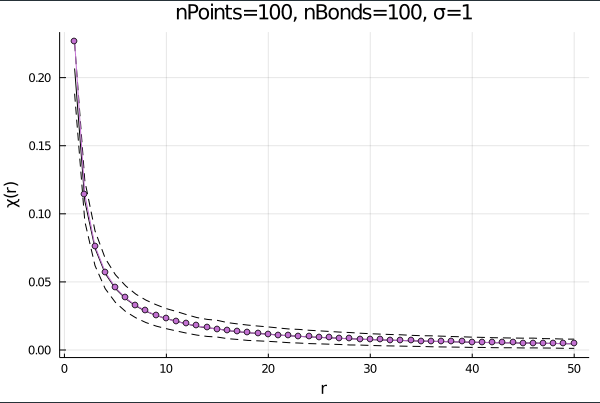
\includegraphics[width=0.8\textwidth]{figures/correlationFunction.png}
%	\caption{The average correlation function (black) $\xi(r)$ and its standard deviation (dashed lines) of  1000 realizations of a connectivity graph with $N=100, nBonds=100, \sigma=1$. In pink, dotted, the fit of the average correlation function to the curve $y = (4.5 r + 0.5) ^ {-1} $.} 
%	\label{fig:correlationFunction}
%\end{figure}
%
% Fig. \ref{fig:nClusters} shows the mean number of clusters and the variation of the mean as a function of $N_l$, for different $\sigma$, as indicated in the legend. The normalized size distribution of the clusters is reported in Fig. \ref{fig:clusterLengthDistribution}.
%
%With a given probability of forming a bond between two nodes that are at a distance $r$ away from each other to be $r^{-\sigma}$, we expect the correlation function $\xi(r)$ (i.e. the distribution of distances at which two nodes are bound) to follow $\sim r^{-\sigma}$. We show in the figure \ref{fig:correlationFunction} the measured average (black, solid line) correlation function and its standard deviation (black, dashed lines) after generating 1000 realizations of the connection graph using Walker's Alias algorithm to draw the bonds among the nodes. In pink, overlayed on top of the black curve, the fit of the average $\xi(r)$ is shown. We fit $\xi(r)$ to the curve $y = (a r + b) ^{-\sigma}$ and obtain a perfect overlay between the data (the average $\xi(r)$) and the fit curve.
%


Fig. \ref{fig:nClusters} displays the number of clusters $N_c$ for different configurations, for constant $N=1024$, as a function of the number of bonds $N_l.$ Different curves correspond to different  $\sigma$, as indicated by the legend. The error bars represent the standard deviation in the sample mean. This is measured from a sample of 100 $J_{ij}$  with the given parameters. Notice the linear behavior of $N_c(N_l)$ for  $N_l < N$, for any value of $\sigma$. Since all possible bonds are free, introduction of a new bond joins two lonely nodes, which destroys a cluster. However, for  $N_l>N$, new bonds will probably join two nodes inside the same cluster, which "slows down" the decay of $N_c.$

Fig. \ref{fig:clusterLengthDistribution} displays the size distribution of the clusters for different $N_l$, for fixed $N.$ The three rows display the distributions for different values of  $\sigma.$ The distributions have been normalised\footnote{With respect to the $L_1$ norm.} for visualization purposes, in order to avoid overrepresentation of distributions skewed to the left\footnote{Notice that for  $N$ spins, there are  $N$ clusters of size 1, and only 1 cluster of size $N$}. Furthermore, since the distributions are skewed to either one of the two boundaries, the left and right columns display zoom-ins of the left and right sides, respectively.

Following \cite{Janke2023}, the order parameter of choice is the magnetization $m = \frac{1}{N}\sum s_i $ of the spin chain. Fig. \ref{fig:magnetization} shows the magnetization of the spin chain, for 50 realizations of the Metropolis algorithm. Each curve is due to a different starting spin seed, and a different $J_{ij}$. The parameters for each Ising run are indicated in the panel title. The averaging of $m^2$ across different runs is reported in Fig. \ref{fig:m2}. In order to compare the behavior for different values of  $N_l$ for constant $\sigma$, Fig. \ref{fig:m2-comparison} displays the superimposition of the different runs, whose parameters are indicated in the panel title, and the legend.

\begin{figure}
	\centering
	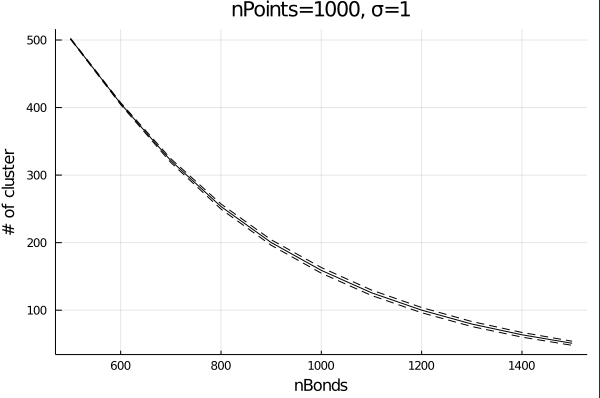
\includegraphics[width=0.8\textwidth]{figures/nClusters.pdf}
	\caption{Average number of clusters and variation of the mean as a function of number of bonds, for $N=1024$ and varying $\sigma$, as indicated by the legend.}
	\label{fig:nClusters}
\end{figure}

\begin{figure}
		\centering
			\includegraphics[width=0.3\textwidth]{figures/ClusterLengthDistributionWithNBonds/zoom-in/Left/nPoints_4096.pdf}
		\includegraphics[width=0.3\textwidth]{figures/ClusterLengthDistributionWithNBonds/nPoints_4096.pdf}
			\includegraphics[width=0.3\textwidth]{figures/ClusterLengthDistributionWithNBonds/zoom-in/Right/nPoints_4096.pdf}
	\caption{In the middle column, the average cluster size distributions (normalised) for fixed number of nodes $N=4096$, for different values of $\sigma$ in the top, middle and bottom panel, as indicated by the label title. The error bars represent the standard error of the sample mean. For visualization purposes, "zoom-ins" of the distributions at the left and right sides of the plot are provided in the left and right columns, respectively.}
	\label{fig:clusterLengthDistribution}
\end{figure}
\begin{figure}[p]
	\hspace{-2cm}
	\begin{subfigure}{1.3\textwidth}
	\includegraphics[width=0.5\textwidth]{figures/Ising Runs/T_0.1_nPoints_4096_nBonds_4096_sigma_0.2.pdf}
	\includegraphics[width=0.5\textwidth]{figures/Ising Runs/T_0.1_nPoints_4096_nBonds_8192_sigma_0.2.pdf}
	\includegraphics[width=0.5\textwidth]{figures/Ising Runs/T_0.1_nPoints_4096_nBonds_4096_sigma_0.8.pdf}
	\includegraphics[width=0.5\textwidth]{figures/Ising Runs/T_0.1_nPoints_4096_nBonds_8192_sigma_0.8.pdf}
	\includegraphics[width=0.5\textwidth]{figures/Ising Runs/T_0.1_nPoints_4096_nBonds_4096_sigma_1.5.pdf}
	\includegraphics[width=0.5\textwidth]{figures/Ising Runs/T_0.1_nPoints_4096_nBonds_8192_sigma_1.5.pdf}
	\end{subfigure}
	\caption{ Magnetization $m$ of the 1-dimensional spin chain with periodic boundary conditions, as iterations of the Metropolis advance, for different spin seeds and $J_{ij}$, for different $\sigma$ and coordination numbers. In the top row, runs of the Metropolis algorithm for $\sigma = 0.2$. In the bottom row, $\sigma = 1.5$. In the left column,  $z = 4$, and thus  $N_l = 2N$. In the right column,  $z = 8$, and thus $N_l = 4N$.}
	\label{fig:magnetization}
\end{figure}
\begin{figure}[p]
	\hspace{-2cm}
	\begin{subfigure}{1.3\textwidth}
	\includegraphics[width=0.5\textwidth]{figures/m2 Runs/T_0.1_nPoints_4096_nBonds_8192_sigma_0.2.pdf}
	\includegraphics[width=0.5\textwidth]{figures/m2 Runs/T_0.1_nPoints_4096_nBonds_16384_sigma_0.2.pdf}
	\includegraphics[width=0.5\textwidth]{figures/m2 Runs/T_0.1_nPoints_4096_nBonds_8192_sigma_1.5.pdf}
	\includegraphics[width=0.5\textwidth]{figures/m2 Runs/T_0.1_nPoints_4096_nBonds_16384_sigma_1.5.pdf}
	\end{subfigure}
	\caption{ Averaged squared magnetization $\left<m^2 \right>$ of the 1-dimensional spin chain with periodic boundary conditions, as iterations of the Metropolis advance, for different spin seeds and $J_{ij}$, for different $\sigma$ and coordination numbers, following the same format as \ref{fig:magnetization}. \textbf{Add linear interpolation}}
	\label{fig:m2}
\end{figure}

\begin{figure}[p]
	\hspace{-2cm}
	\begin{subfigure}{1.3\textwidth}
	\includegraphics[width=0.5\textwidth]{figures/m2 Runs/Sigma groupings/T_0.1_nPoints_4096_sigma_0.2.pdf}
	\includegraphics[width=0.5\textwidth]{figures/m2 Runs/Sigma groupings/T_0.1_nPoints_8192_sigma_0.2.pdf}
	\includegraphics[width=0.5\textwidth]{figures/m2 Runs/Sigma groupings/T_0.1_nPoints_4096_sigma_0.8.pdf}
	\includegraphics[width=0.5\textwidth]{figures/m2 Runs/Sigma groupings/T_0.1_nPoints_8192_sigma_0.8.pdf}
	\includegraphics[width=0.5\textwidth]{figures/m2 Runs/Sigma groupings/T_0.1_nPoints_4096_sigma_1.5.pdf}
	\includegraphics[width=0.5\textwidth]{figures/m2 Runs/Sigma groupings/T_0.1_nPoints_8192_sigma_1.5.pdf}
	\end{subfigure}
	\caption{Comparison of the averaged $m^2$ for different $N_l$, with $N, T, \sigma$ as indicated y the title of the panel and $N_l$ indicated by the legend. \textbf{Add linear interpolation}}
	\label{fig:m2-comparison}
\end{figure}



\newpage
%\section{Literature notes -- To be deleted}

\paragraph{Notes on Monte Carlo algorithms}
Given a partition function 
\begin{align}
	Z = \sum_s \exp{(-i\beta E_s)},
\end{align}
the calculation of thermodynamic observables is extremely computationally expensive, as one has to integrate over the whole phase space.
To avoid this, the Monte Carlo method of integration is used, based on the idea of trial and error, from Markov chains. The key characteristic of these chains is that each element \textbf{only} depends on the previous element.

Starting from a configuration $s_i$ with a non vanishing Boltzmann factor $p_i$, a new trial configuration $s_j$ is created with Boltzmann factor $p_j$. 
From each state $s_i$ to $s_j$ there is a transition probability represented by a transition matrix $\pi_{ij}$. One looks for the transition matrix yielding the equilibrium distribution $p_j$, so that 
\begin{align}
	\sum_i p_i \pi_{ij} = p_j.
	\label{eq:equilibrium-condition}
\end{align}
One looks for the solutions $\pi_{ij}$ by imposing the condition of \textit{microscopic reversibility} or \textit{detailed balance}
\begin{align}
	p_i \pi_{ij} = p_j \pi_{ji}.
	\label{eq:microscopic-reversibility}
\end{align}
Equations \eqref{eq:equilibrium-condition} and \eqref{eq:microscopic-reversibility} are equivalent if
\begin{align}
	\sum_i \pi_{ji} = 1.
\end{align}
We split each $\pi_{ij}$ as the product of an \textit{a priori} transition probability $\alpha_{ij}$ of generating $s_j$ from $s_i$ and an acceptance probability $P_{ij}$ of accepting $s_j$ as the new state. We thus write \eqref{eq:microscopic-reversibility} as 
\begin{align}
	p_i \alpha_{ij} P_{ij} = p_j \alpha_{ji} P_{ji}.
\end{align}
If $\alpha$ is symmetric, 
\begin{align}
	\frac{P_{ij}}{P_{ji}} = \exp[ - \beta ( E_j - E_i)].
\end{align}
This does not uniquely define $P$. \cite{Metropolis1953} suggests 
\begin{align}
	\frac{P_{ij}}{P_{ji}} = 
	\begin{cases}
		\exp{-\beta (E_j - E_i)} & E_j > E_i \\
		1 & E_j \leq E_i.
		\end{cases}
\end{align}
This way, thermodynamic averages are calculated by generating a sequence of $M$ configurations $\{ s_1, \ldots s_M \}$, 
\begin{align}
	\langle A \rangle \approx \frac{1}{M} \sum_{n=1 }{M}A_n.
\end{align}

The Ising model is modelled by the Hamiltonian
\begin{align}
	\mathcal{H}_\text{Ising} = -J \sum_{\langle ij \rangle} s_i s_j.
\end{align}),
where the sum runs over all pairs of neares neighbors, coupled via ferromagnetic coupling with strength $J>0$. Local trial moves correspond to flipping single spins.

\cite{PhysRevLett.58.86} changes the Monte carlo
algorithm from a ``single-spin flip''. The recipe of this algorithm is as follows:

\begin{enumerate}
	\item A ``bond'' is formed between every pair of nearest neighbors,aligned with a probability $p_{ij} = 1 - \exp(-i\beta J)$, with $J$ the coupling constant.
	\item Connected bonds (directly or indirectly) belong to the same cluster\footnote{They supposedly have the same spin? From \cite{Luijten2006}: ``The bond assignment procedure divides the system into clusters of \textit{parallel} spins (a so-called cluster decomposition) [...] two spins of the same sign need not belong to the same cluster, even if these spins are adjacent on the lattice. }
	\item Spins in each cluster are flipped collectively with probability $\frac{1}{2}$. 
	\item Delete all bonds, perform step (1) again.
\end{enumerate}

This algorithm suppresses the dynamic slowing down near critical points. Near critical points (continuous phase transitions), the relaxation time of thermodynamic properties depends on the correlation length 
\begin{align}
	\tau \propto \xi ^z,
\end{align}
with $z\approx2$ the so-called dynamical critical exponent. The correlation length diverges as 
\begin{align}
	\xi \propto \lvert T - T_c \rvert ^{-\nu},
\end{align}
with $\nu > 0 $. As $T\to T_c$, we encounter a \textit{critical slowing down}. Larger systems with larger correlation lengths present larger correlation times, and it therefore becomes increasingly difficult to generate statistically independent configurations. 

The above mentioned algorithm destroys nonlocal correlations, and the dynamical exponent $z$ is lowered to a much smaller value. 


\newpage
\appendix
\section{Code snippets}%
\label{sec:Code for the connection set method}

\subsection{Code for the generation of connection sets}%
\label{sub:Code for the generation of connection sets}

\begin{lstlisting}


using AliasTable

function generateConnectionsSet(N, N_l, sigma)

    distancesArray = 1:(N-1)
    chooseAT = AliasTable(ones(nPoints))
    distanceAliasTable = AliasTable(
   		 1 ./ distancesArray .^ (1+sigma)
		 )

    # Stores connections
    connectionsSet = Set() 

    # Stops if N_l is reached
    while len(connectionsSet) < N_l
	# Uniform distribution
        particle1Choice = rand(chooseAT, 1)[1]

	# Rolls integer m with probability P_m = m^(-(1+sigma))
        particle2Addition = rand(distanceAliasTable, 1)[1]
        particle2Choice = (particle2Addition + particle1Choice) % N

	# Stores the sampled connection. Since sets do not repeat elements 
	# and are also unordered, if the connection already existed,
	# it will not be stored.
        push!(connectionsSet, 
		Set([particle1Choice, particle2Choice]))
    end
    connectionsSet
end

\end{lstlisting}



\subsection{Code for the clustering algorithms}%
\label{sub:code for the clustering algorithms}
\begin{lstlisting}
function clusterIdentification(connectivityArray)
    nPoints = length(connectivityArray)
    visited = Set{Int}()
    clusters = []

    function dfs(node, cluster)
        stack = [ node ]
        while !isempty(stack)
            curr = pop!(stack)
            if !(curr in visited)
                push!(visited, curr)
                push!(cluster, curr)
                for neighbor in connectivityArray[curr]
                    if !(neighbor in visited)
                        push!(stack, neighbor)
                    end
                end
            end
        end
        cluster
    end

        for i in 1:nPoints
            if !(i in visited)
                cluster = Set{Int}()
                cluster = dfs(i, cluster)
                append!(clusters, [cluster])
            end
        end
        length(clusters)
end
	
\end{lstlisting}





\newpage
\bibliographystyle{abbrvnat}
\bibliography{notes}

\end{document}
